%!Tex Program = xelatex
%\documentclass[a4paper]{article}
\documentclass[a4paper]{ctexart}
\usepackage{xltxtra}
%\setCJKmainfont{Noto Serif CJK SC} 
%\setCJKmainfont{AR PL UMing CN:style=Light}
%\setmainfont[Mapping=tex-text]{AR PL UMing CN:style=Light}
%\setmainfont[Mapping=tex-text]{AR PL UKai CN:style=Book}
%\setmainfont[Mapping=tex-text]{WenQuanYi Zen Hei:style=Regular}
%\setmainfont[Mapping=tex-text]{WenQuanYi Zen Hei Sharp:style=Regular}
%\setmainfont[Mapping=tex-text]{AR PL KaitiM GB:style=Regular} 
%\setmainfont[Mapping=tex-text]{AR PL SungtiL GB:style=Regular} 
%\setmainfont[Mapping=tex-text]{WenQuanYi Zen Hei Mono:style=Regular} 

\usepackage{listings}
\usepackage{xcolor}
\usepackage{graphicx}
\usepackage{amsmath}
\usepackage{amsthm}
\usepackage{amssymb}
\usepackage{mathrsfs}
\definecolor{codegreen}{rgb}{0,0.6,0}
\definecolor{codegray}{rgb}{0.5,0.5,0.5}
\definecolor{codepurple}{rgb}{0.58,0,0.82}
\definecolor{backcolour}{rgb}{0.95,0.95,0.92}

\renewcommand{\thefigure}{\arabic{section}.\arabic{figure}}

\lstdefinestyle{mystyle}{
    backgroundcolor=\color{backcolour},   
    commentstyle=\color{codegreen},
    keywordstyle=\color{magenta},
    numberstyle=\tiny\color{codegray},
    stringstyle=\color{codepurple},
    basicstyle=\ttfamily\footnotesize,
    breakatwhitespace=false,         
    breaklines=true,                 
    captionpos=b,                    
    keepspaces=true,                 
    numbers=left,                    
    numbersep=5pt,                  
    showspaces=false,                
    showstringspaces=false,
    showtabs=false,                  
    tabsize=2
}

\lstset{style=mystyle}

\newcommand{\hl}[1]
{\noindent {\bf {#1}}}

% 创建定理环境  
\newtheorem{theorem}{定理}  

\theoremstyle{definition}  
\newtheorem{definition}{定义}[section]

\theoremstyle{definition}  
\newtheorem{example}{例}[section]  


\title{数据结构和算法}
\author{}
\date{}
\begin{document}
\maketitle
\pagestyle{empty}

\setcounter{section}{4}
\section{散列表}

我们已经学习了平衡树, 这是一种能使我们的全部操作都保持 $\Theta(\log
n)$ 效率的数据结构(最坏情形或平摊情形). 在这个基础上, 一个显然的问题
是: 我们还能效率再高一点么? 比如: 对所有操作, 其最坏情形或者至少平摊情
形是 $\Theta(1)$ ? 那就意味着任何一个单步操作, 不论是查找, 插入还是删
除, 都只需要常数时间, 或者说, 其操作时间和数据集本身的大小无关. 当数据
规模趋于无穷时(或充分大时), 这些基本操作所需的时间不变. 直觉告诉我们,
即便对平摊情形, 这也是不可能的. 但是, 我们能否在一些具体的限制条件下
(比如数据总量是有确定上界的, 而且这个上界不会导致我们系统的内存溢出),
在部分基本操作上(比如至少查找, 插入和删除这三个最基本操作), 满足单个操
作是 $\Theta(1)$ 的效率? 我们这一章给出一种数据结构, 来逼近这一要求.
之所以说逼近, 是因为在实际操作中, 你必须比较小心各种限制, 才能真正实现
这个目的.

在第4章中，我们讨论了搜索树 ADT，它允许对一组元素进行各种操作。在本章中，我们讨论散列表 ADT，它只支持二叉搜索树所允许的操作的一个子集。

散列表的实现通常称为哈希。哈希是一种用于执行插入、删除和查找的技术，平均时间复杂度为常数。需要对元素进行排序的操作效率不高。
因此，诸如 \verb|findMin|、\verb|findMax| 以及在线性时间内按排序顺序打印整个表的操作是不支持的。

本章的核心数据结构是散列表。我们将...

\begin{itemize}
    \item 看到几种实现散列表的方法。
    \item 从分析的角度比较这些方法。
    \item 展示哈希的多种应用。
    \item 比较散列表与二叉搜索树。
\end{itemize}

\subsection{总体概念}
% 5.1

理想的散列表数据结构仅仅是一个包含项的固定大小的数组。如第4章所讨论的，通常在项的某个部分（即数据成员）上执行搜索。
这被称为键。例如，一个项可能由一个字符串（作为键）和附加的数据成员组成（例如，一个名字是大型员工结构的一部分）。
我们将表的大小称为 \texttt{TableSize}，理解这是哈希数据结构的一部分，而不仅仅是一些全局浮动的变量。
通常的约定是让表从 0 到 \texttt{TableSize-1} 运行；我们很快就会看到原因。

每个键都被映射到 0 到 \texttt{TableSize-1} 范围内的某个数字，并放置在适当的单元格中。
这种映射被称为哈希函数，理想情况下应该简单易算，并确保任何两个不同的键得到不同的单元格。
由于单元格数量有限而键的供应几乎是无穷无尽的，这显然是不可能的，因此我们寻求一个哈希函数，
将键均匀分布在单元格中。

$$
h(key) \to x, \quad 0 \leq x < T - 1, key \in \text{key space}.
$$

图5.1 是一个完美情况的典型例子。在这个例子中，john哈希到3，phil哈希到4，dave哈希到6，mary哈希到7。

\begin{center}
    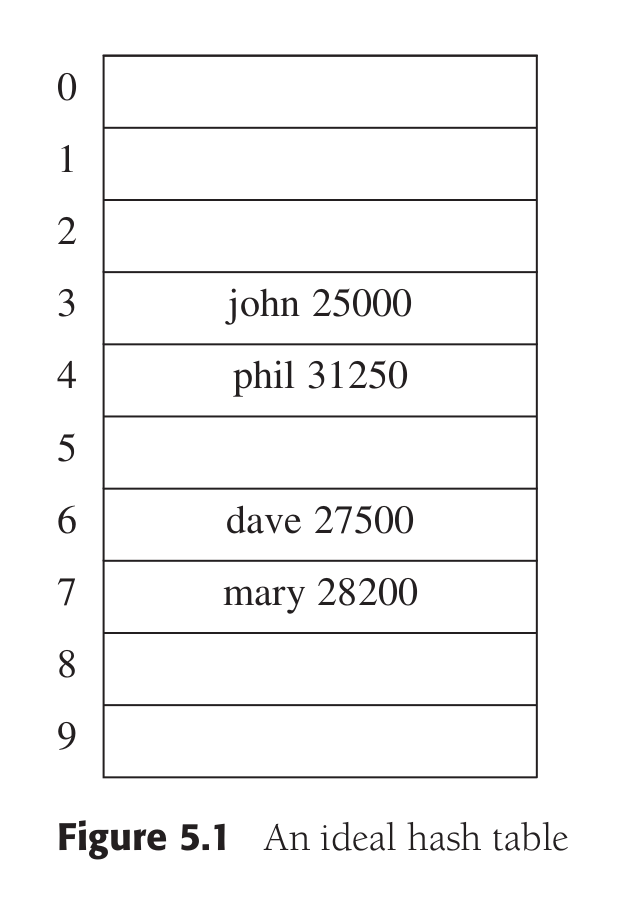
\includegraphics[width=0.3\textwidth]{images/hash_example.png}
\end{center}

这就是哈希的基本概念。唯一剩下的问题包括选择一个函数，决定当两个键哈希到同一个值时该怎么做（这被称为碰撞），以及决定表的大小。

\subsection{哈希函数}
% 5.2

% 如果输入的键是整数，那么简单地返回\texttt{Key mod TableSize}通常是一个合理的策略，除非\texttt{Key}碰巧有一些不理想的特性。
% 在这种情况下，哈希函数的选择需要仔细考虑。例如，如果表大小是 10 而键都以零结尾，那么标准哈希函数是一个不好的选择。
% 出于我们将在后面看到的原因，为了避免上述情况，通常最好确保表大小是素数。当输入键是随机整数时，这个函数不仅非常简单易算，而且还能均匀分布键。

首先是表的大小，按照上节课我们讨论过的情况，我们将表的大小定为素数。我们来看一些最简单的实现。

通常，键是具有唯一性的字符串；在这种情况下，哈希函数需要仔细选择。一个选择是将字符串中字符的ASCII值相加。图5.2中的例程实现了这种策略。
然后通过取模使结果落在表的范围内。这个函数简单易算，而且对于随机字符串，它通常能很好地分布键。

\begin{lstlisting}[language=C++]
int hash( const string & key, int tableSize )
{
  int hashVal = 0;
  for( char ch : key )
    hashVal += ch;
  return hashVal % tableSize;
}
\end{lstlisting}  

图5.2中描述的哈希函数简单易实现，并且能快速计算出答案。然而，如果表大小很大，该函数不能很好地分布键。
例如，假设\texttt{TableSize = 10,007}（10,007是一个素数）。假设所有键都是八个或更少字符长。
由于一个ASCII字符有一个整数值，该值总是最多 127，（英文！）哈希函数通常只能假设值在 0 到 1,016 之间，即\(127 \times 8\). 
这显然不是一个公平的分布！

另一个哈希函数显示在图 5.3 中。这个哈希函数假设\texttt{Key}至少有三个字符。值27代表英文字母表中字母的数量，加上空格，而 729 是\(27^2\)。
见过 27 进制么？
\begin{lstlisting}[language=C++]
int hash( const string & key, int tableSize )
{
  return ( key[ 0 ] + 27 * key[ 1 ] + 729 * key[ 2 ] ) % tableSize;
}  
\end{lstlisting}
这个函数只检查前三个字符，但如果这些是随机的，并且表大小是 10,007，和之前一样，那么我们期望一个合理的公平分布。
不幸的是，英语不是随机的。虽然有三个字符（忽略空格）的\(26^3 = 17,576\) 种可能组合，但检查一个相当大的在线词典显示，
不同组合的数量实际上只有 2,851。即使这些组合没有冲突，也只有28 \%的表可以实际被哈希到。
因此，这个函数，尽管容易计算，但如果哈希表相当大，也是不合适的。

图5.4显示了第三种哈希函数的尝试。这个哈希函数涉及键中的所有字符，并且可以预期会很好地分布
（它计算\(\sum_{i=0}^{\text{KeySize}-1} \text{Key[KeySize} - i - 1] \cdot 37^i\)并将结果带入适当的范围）。
代码通过使用 Horner 规则计算一个多项式。例如，另一种计算\(h_k = k_0 + 37k_1 + 37^2k_2\) 的方法是使用公式 \(h_k = ((k_2) \times 37 + k_1) \times 37 + k_0\)。
Horner规则将此扩展到 n 次多项式。

\begin{lstlisting}[language=C++]
/**
 * A hash routine for string objects.
*/
unsigned int hash( const string & key, int tableSize )
{
  unsigned int hashVal = 0;
  for( char ch : key )
    hashVal = 37 * hashVal + ch;
  return hashVal % tableSize;
//  ((key[0] * 37 + key[1]) * 37 + key[2]) * 37 + key[3]  
  }  
\end{lstlisting}

为啥 37? 素数！顺便说一下，Horner 规则在中国叫秦九韶算法，是中国古代的一种多项式求值算法。秦九韶是一个人！这个算法出现在他的作品《数书九章》
（不是《九章算术》，这个在汉代，里面提到了类似的思想，但不完整）中。
秦九韶是南宋人，但可以认为是浙大校友！因为他设计了西溪校区门口的道古桥。

哈希函数利用了允许溢出并使用无符号整数来避免引入负数的事实。

图5.4中描述的哈希函数不一定在表分布方面是最好的，但它具有极端简单性的优点，
并且计算速度相当快。如果键非常长，哈希函数将花费太长时间来计算。在这种情况下，
通常的做法是不全用所有的字符。键的长度和属性将影响选择。例如，键可能是一个完整的街道地址。
哈希函数可能包括来自街道地址的几个字符，以及可能来自城市名称和邮政编码的几个字符。
一些程序员通过仅使用奇数位置的字符来实现他们的哈希函数，
其想法是节省计算哈希函数的时间将弥补稍微不均匀分布的函数。

主要的编程细节是冲突解决。如果插入一个元素时，它与已经插入的元素具有相同的哈希值，
那么我们就有了冲突，需要解决它。有几种方法可以处理这个问题。我们将讨论两种最简单的方法：
分离链接和开放寻址；然后我们将看看一些最近发现的替代方法。

\subsection{分离链接}
% 5.3

第一种策略，通常称为分离链接，是保留所有具有相同哈希值的元素的列表。我们可以使用标准库 \verb|list| 实现。
如果空间紧张，可能更倾向于避免使用它们（因为这些 list 是双向链接的，并且浪费空间）。
在本节中，我们假设键是前10个完全平方数，并且哈希函数简单地为 $\text{hash}(x) = x \mod 10$。
（表大小不是素数，但出于简单起见，这里使用它。）图5.5显示了结果的分离链接哈希表。

\begin{center}
  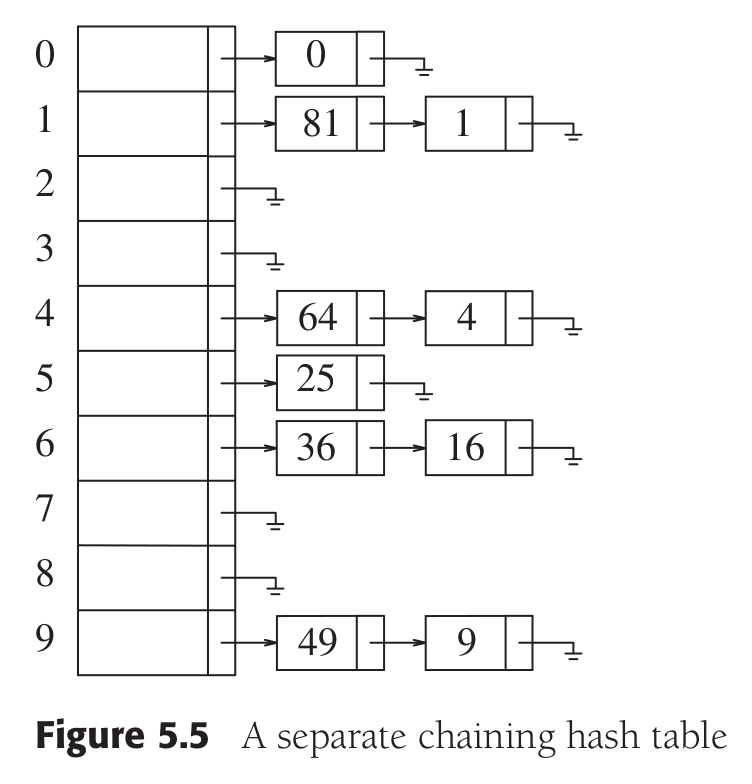
\includegraphics[width = 0.5 \textwidth]{images/seprate_chaining.png}
\end{center}

为了执行搜索，我们使用哈希函数来确定要遍历哪个列表。然后搜索适当的列表。为了执行插入，
我们检查适当的列表，看看元素是否已经存在（如果期望有重复项，则通常保留一个额外的数据成员，并在匹配时递增该数据成员）。
如果元素是新的，它可以插入到列表的前面，因为这样很方便，而且经常发生最近插入的元素是最有可能在不久的将来被访问的元素。

分离链接实现的类接口如图5.6所示。哈希表存储一个链表数组，这些链表在构造函数中分配。

\begin{lstlisting}
template <typename HashedObj>
class HashTable
{
public:
  explicit HashTable( int size = 101 );
  bool contains( const HashedObj & x ) const;
  void makeEmpty( );
  bool insert( const HashedObj & x );
  bool insert( HashedObj && x );
  bool remove( const HashedObj & x );
private:
  vector<list<HashedObj> > theLists;
  int currentSize;
  // The array of Lists
  void rehash( );
  size_t myhash( const HashedObj & x ) const;
};  
\end{lstlisting}

类接口说明了 C++11 之前的一个语法点：在声明列表时，两个 \verb|>| 之间需要一个空格；因为 \verb|>>| 是C++的标记，
并且因为它比 \verb|>| 长，所以 \verb|>>| 将被识别为标记。在 C++11 中，情况不再是这样。

正如二叉搜索树只适用于可比较的对象一样，本章中的哈希表只适用于提供哈希函数和等价操作符（操作符==或操作符!=，或可能两者都有）的对象。

我们不再要求哈希函数同时接受对象和表大小作为参数，而是让我们的哈希函数只接受对象作为参数并返回适当的整型。
这样做的标准机制使用函数对象，哈希表的协议在C++11中引入。具体来说，在C++11中，哈希函数可以通过函数对象模板来表示：

\begin{lstlisting}
template <typename Key>
class hash
{
  public:
  size_t operator() ( const Key & k ) const;
};
\end{lstlisting}

也就是说这是一个模板类，它有一个 \verb|operator()| 函数，它接受一个键并返回一个 \verb|size_t|。这个类的实例可以用作哈希表的哈希函数。

默认为标准类型如 \verb|int| 和 \verb|string| 提供了此模板的实现；因此，图5.4中描述的哈希函数可以如下实现：

\begin{lstlisting}[language=C++]
template <>
class hash<string>
{
public:
    size_t operator()( const string & key )
    {
        size_t hashVal = 0;

        for( char ch : key )
            hashVal = 37 * hashVal + ch;

        return hashVal;
    }
};
\end{lstlisting}

类型 \verb|size\_t| 是一个无符号整型，代表一个对象的大小；因此，它保证能够存储一个数组索引。
实现哈希表算法的类可以调用通用哈希函数对象来生成一个整型 \verb|size\_t|，然后将结果缩放到一个合适的数组索引。
在我们的哈希表中，这体现在图5.7中显示的私有成员函数 \verb|myhash|中。

\begin{lstlisting}[language=C++]
size_t myhash( const HashedObj & x ) const
{
  static hash<HashedObj> hf;
  return hf( x ) % theLists.size( );
}  
\end{lstlisting}

图5.8展示了一个 \verb|Employee| 类，它可以存储在通用哈希表中，使用 \verb|name| 成员作为键。\verb|Employee|
类通过提供等价操作符和一个哈希函数对象实现了 \verb|HashedObj| 要求。

\begin{lstlisting}[language=C++]
// Example of an Employee class
class Employee
{
public:
  const string & getName( ) const
  { return name; }
  bool operator==( const Employee & rhs ) const
  { return getName( ) == rhs.getName( ); }
  bool operator!=( const Employee & rhs ) const
  { return !( *this == rhs); }
  // Additional public members not shown
private:
  string name;
  double salary;
  int seniority;
  // Additional private members not shown
};
  
template<>
class hash<Employee>
{
public:
  size_t operator()( const Employee & item )
  {
    static hash<string> hf;
    return hf( item.getName( ) );
  }
};
\end{lstlisting}

这份代码只是一个示例。

实现 \verb|makeEmpty|、\verb|contains| 和 \verb|remove| 的代码如图5.9所示。

接下来是插入例程。如果待插入的项目已经存在，那么我们什么也不做；
否则，我们将其放入列表中（见图5.10）。元素可以放在列表中的任何位置；
使用 \verb|push\_back| 在大多数情况下是最方便的，\verb|whichList| 是一个引用变量；关于这种使用引用变量的讨论，
请参见第1.5.2节。

除了使用链表来解决冲突之外，还可以使用任何方案；
二叉搜索树甚至另一个哈希表都可以工作，但我们期望如果表很大并且哈希函数很好，所有列表都应该很短，
因此基本的分离链接不会尝试任何复杂的东西。

我们定义哈希表的负载因子 $\lambda$ 为哈希表中的元素数量与表大小的比率。在上面的例子 (Fig 5.5) 中，$\lambda = 1.0$. 
列表的平均长度是 $\lambda$. 执行搜索所需的努力是评估哈希函数所需的常数时间加上遍历列表的时间。
在不成功的搜索中，需要检查的节点数量平均是 $\lambda$. 一个成功的搜索需要遍历大约 $1 + (\lambda/2)$ 个链接。
为了理解这一点，请注意正在搜索的列表包含存储匹配项的一个节点加上零个或多个其他节点。
在具有 $N$ 个元素和 $M$ 个列表的表中， ``其他节点'' 的预期数量是 $(N - 1)/M = \lambda - 1/M$, 
这基本上就是 $\lambda$, 因为 $M$ 被假定为很大。平均而言，一半的 ``其他节点'' 被搜索，因此结合匹配节点，
我们得到平均搜索成本(期望)为 $1 + \lambda/2$ 个节点。这个分析表明，表的大小并不是很重要，
但负载因子是。分离链接哈希的一般规则是使表大小大约与预期的元素数量一样大
（换句话说，让 $\lambda \approx 1$）。在图 5.10 中的代码中，如果负载因子超过 $1$，
我们通过在第10行调用 \verb|rehash| 来扩展表大小。\verb|rehash| 在第5.5节中讨论。如前所述，
保持表大小为素数也是一个好主意，以确保良好的分布。

上周我们讨论散列表就像同学们在教室中找座位一样，如果发现冲突，直接坐腿上大家都觉得很变态。但刚刚大家接受的分离链表法，
本质上就是接受了这个方案。那么有没有不那么变态的方案呢？

\subsection{无链表的哈希表}
% 5.4

分离链接哈希的缺点是使用链表。这可能会因为分配新单元格所需的时间（尤其是在其他语言中）而稍微减慢算法速度，并且基本上需要实现第二种数据结构。
解决与链表冲突的替代方法是尝试其他单元格直到找到一个空单元格。更正式地说，单元格$h_0(x), h_1(x), h_2(x), \ldots$被依次尝试，
其中$h_i(x) = (\text{hash}(x) + f(i)) \mod \text{TableSize}$，$f(0) = 0$. 
函数$f$是冲突解决策略。因为所有数据都进入表中，所以在这种方案中需要一个比分离链接哈希更大的表。
通常，对于不使用分离链接的哈希表，负载因子应低于$\lambda = 0.5$. 我们称这样的表为探测哈希表。
我们现在来看三种常见的冲突解决策略。

\subsubsection{线性探测}
% 5.4.1 

在线性探测中，$f$是$i$的线性函数，通常是$f(i) = i$. 这相当于尝试单元格序列（带环绕）以寻找空单元格。
图5.11显示了使用与之前相同的哈希函数 (\verb|mod 10|) 和冲突解决策略 $f(i) = i$ 将键 \{89, 18, 49, 58, 69\} 插入哈希表的结果。

当 49 被插入时，第一次冲突发生；它被放入下一个可用位置，即位置 0 ，该位置是空的。
键 58 与 18 和 89 发生冲突，然后 49 在三个位置之后找到一个空单元格。
69 的冲突以类似方式处理。只要表足够大，总能找到空单元格，但这样做的时间可能会变得很长。
更糟糕的是，即使表相对空，占用单元格的块也会开始形成。这种效应，称为初级聚集，
意味着任何哈希到该簇的键都将需要几次尝试来解决冲突，然后它将添加到该簇中。

虽然我们这里不会执行计算，但可以证明，使用线性探测的预期探测次数大约为 
$$
\frac{1}{2}(1 + \frac{1}{(1 - \lambda)^2})
$$
用于插入和不成功的搜索，以及
$$
\frac{1}{2}(1 + \frac{1}{(1 - \lambda)})
$$
用于成功的搜索。计算有些复杂。从代码中很容易看出，插入和不成功的搜索需要相同数量的探测。
片刻的思考表明，平均而言，成功的搜索应该比不成功的搜索花费更少的时间。

\subsubsection{二次探测}
% 5.4.2

二次探测是一种消除线性探测主要聚集问题的冲突解决方法。正如你所期望的，二次探测的冲突函数是二次的。一个流行的选择是$f(i) = i^2$. 
图5.13展示了使用这个冲突函数在与线性探测示例相同的输入上得到的哈希表结果。

当 49 与 89 发生冲突时，下一个尝试的位置是相邻的单元格。这个单元格是空的，所以 49 被放置在那里。
接下来，58 在位置 8 发生冲突。然后，相邻的单元格被尝试，但另一个冲突发生了。在尝试下一个单元格时发现了一个空单元格，
该单元格距离为$2^2 = 4$. 因此，58 被放置在单元格 2 中。69 也发生了同样的情况。

对于线性探测，让哈希表几乎满是一个坏主意，因为性能会下降。对于二次探测，情况更加严重：一旦表超过半满，甚至在表大小不是素数的情况下，
在表半满之前，就没有保证能找到一个空单元格。这是因为在表的一半中，最多可以使用作为解决冲突的替代位置。

实际上，我们现在可以证明，如果表是半空的，并且表大小是素数，那么我们总是能够插入一个新元素。

\noindent \textbf{定理 5.1} 如果使用二次探测，并且表大小是素数，那么只要表至少有一半是空的，总是可以插入一个新元素。

\begin{proof}
设表大小，$\text{TableSize}$, 是一个大于 $3$ 的奇数素数。我们证明前 $[\text{TableSize}/2]$ 个替代位置
（包括初始位置$h_0(x)$）
都是不同的。其中两个位置是 $h(x) + i^2 \pmod{\text{TableSize}}$ 和 $h(x) + j^2 \pmod{\text{TableSize}}$，
任取其中$0 \leq i, j \leq [\text{TableSize}/2]$. 假设，为了矛盾，这些位置相同，但$i \neq j$. 那么
\begin{align*}
  h(x) + i^2 &\equiv h(x) + j^2 \pmod{\text{TableSize}} \\
  i^2 &\equiv j^2 \pmod{\text{TableSize}} \\
  i^2 - j^2 &\equiv 0 \pmod{\text{TableSize}} \\
  (i - j)(i + j) &\equiv 0 \pmod{\text{TableSize}}
\end{align*}
  
由于$\text{TableSize}$是素数，因此要么$(i - j)$要么$(i + j)$等于 $0$（模$\text{TableSize}$）。
由于$i$和$j$是不同的，第一种情况是不可能的。由于$0 \leq i, j \leq [\text{TableSize}/2]$, 
第二种情况也是不可能的。因此，前$[\text{TableSize}/2]$个替代位置是不同的。
如果最多$[\text{TableSize}/2]$个位置被占用，那么足够多次尝试后总能找到空位。
\end{proof}

如果表甚至超过半满，插入可能会失败（尽管这种情况极不可能）。因此，重要的是要记住这一点。同样重要的是，
表大小必须是素数。如果表大小不是素数，替代位置的数量可能会大大减少。例如，如果表大小为16，那么唯一的替代位置将在距离1、4或9处。

在探测哈希表中不能执行标准删除，因为单元格可能已经引起了冲突，使其无法通过。
例如，如果我们删除89，那么几乎所有的find操作都会失败。因此，探测哈希表需要延迟删除，
尽管在这种情况下实际上并没有延迟。

实现探测哈希表所需的类接口如图5.14所示。我们不是使用列表数组，而是使用哈希表条目单元格的数组。
嵌套类HashEntry存储信息成员中条目的状态；这个状态可以是ACTIVE、EMPTY或DELETED。

我们使用一个标准的枚举类型。

\begin{lstlisting}[language=C++]
enum EntryType { ACTIVE, EMPTY, DELETED };
\end{lstlisting}

构建表（图5.15）包括为每个单元格将info成员设置为EMPTY。contains(x)，如图5.16所示，涉及私有成员函数isActive和findPos。
私有成员函数findPos执行冲突解决。我们在插入例程中确保哈希表至少是表中元素数量的两倍，因此二次解决总是有效的。
在图5.16中，被标记为已删除的元素计为在表中。这可能会导致问题，因为表可能会过早地变得太满。我们将在本章后面讨论这个问题。

第12至15行表示进行二次解决的快速方法。根据二次解决函数的定义，$f(i) = f(i - 1) + 2i - 1$，
所以下一个要尝试的单元格是从之前尝试的单元格开始的距离，并且这个距离在连续探测中每次增加2。

\begin{lstlisting}[language=C++]
template <typename HashedObj>
class HashTable
{
public:
  explicit HashTable( int size = 101 );
  bool contains( const HashedObj & x ) const;
  void makeEmpty( );
  bool insert( const HashedObj & x );
  bool insert( HashedObj && x );
  bool remove( const HashedObj & x );
  enum EntryType { ACTIVE, EMPTY, DELETED };
private:
  struct HashEntry
  {
    HashedObj element;
    EntryType info;
    HashEntry( const HashedObj & e = HashedObj{ }, EntryType i = EMPTY )
    : element{ e }, info{ i } { }
    HashEntry( HashedObj && e, EntryType i = EMPTY )
    : element{ std::move( e ) }, info{ i } { }
  };
  vector<HashEntry> array;
  int currentSize;
  bool isActive( int currentPos ) const;
  int findPos( const HashedObj & x ) const;
  void rehash( );
  size_t myhash( const HashedObj & x ) const;
};  
\end{lstlisting}

如果新位置超出了数组范围，可以通过减去$\text{TableSize}$将其放回范围内。这比明显的方法更快，因为它避免了似乎需要的乘法和除法。
一个重要的警告：第9行和第10行的测试顺序很重要。不要改变它！

最后的例程是插入。如果$x$已经存在，我们不做任何事情。这是一个简单的修改，可以做一些其他事情。否则，
我们将其放在$\text{findPos}$例程建议的位置。代码显示在图5.17中。如果负载因子超过0.5，表就满了，我们扩大哈希表。这称为rehashing，并在第5.5节中讨论。图5.17还显示了remove。

\begin{lstlisting}[language=C++]
explicit HashTable( int size = 101 ) : array( nextPrime( size ) )
{ makeEmpty( ); }
  
void makeEmpty( )
{
  currentSize = 0;
  for( auto & entry : array )
    entry.info = EMPTY;
}  
\end{lstlisting}

\begin{lstlisting}[language=C++]
bool contains( const HashedObj & x ) const
{ return isActive( findPos( x ) ); }

int findPos( const HashedObj & x ) const
{
  int offset = 1;
  int currentPos = myhash( x );
  
  while( array[ currentPos ].info != EMPTY &&
         array[ currentPos ].element != x )
  {
    currentPos += offset; // Compute ith probe
    offset += 2;
    if( currentPos >= array.size( ) )
      currentPos-= array.size( );
  }
  
  return currentPos;
}

bool isActive( int currentPos ) const
{ return array[ currentPos ].info == ACTIVE; }  
\end{lstlisting}

虽然二次探测消除了初级聚集，但哈希到同一位置的元素将探测相同的替代单元格。这被称为次级聚集。次级聚集是一个轻微的理论问题。
模拟结果表明，它通常导致每次搜索多于半个探测。以下技术消除了这一点，但代价是计算一个额外的哈希函数。

\begin{lstlisting}[language=C++]
bool insert( const HashedObj & x )
{
  // Insert x as active
  int currentPos = findPos( x );
  if( isActive( currentPos ) )
    return false;
  
  array[ currentPos ].element = x;
  array[ currentPos ].info = ACTIVE;
  
  // Rehash; see Section 5.5
  if( ++currentSize > array.size( ) / 2 )
    rehash( );
  
  return true;
}

bool remove( const HashedObj & x )
{
  int currentPos = findPos( x );
  if( !isActive( currentPos ) )
    return false;
  
  array[ currentPos ].info = DELETED;
  return true;
}
\end{lstlisting}

\subsubsection{双重哈希}
% 5.4.3 

我们将要研究的最后一个冲突解决方法是双重哈希。对于双重哈希，
一个流行的选择是 $f(i) = i \cdot \text{hash}_2(x)$. 
这个公式说我们对$x$应用第二个哈希函数，并在距离 
$\text{hash}_2(x), 2\text{hash}_2(x), \ldots$ 处探测。
选择 $\text{hash}_2(x)$ 的一个糟糕选择将是灾难性的。
例如，明显选择$\text{hash}_2(x) = x \mod 9$ 如果99被插入到前面例子的输入中将不会有帮助。
因此，函数绝不能评估为零。同样重要的是要确保所有单元格都可以被探测（这在下面的例子中是不可能的，因为表大小不是素数）。
这样一个函数是 $\text{hash}_2(x) = R - (x \mod R)$，其中$R$是一个小于$\text{TableSize}$的素数，
将会很好地工作。如果我们选择$R = 7$，那么图5.18显示了像以前一样插入相同键的结果。

\begin{center}
  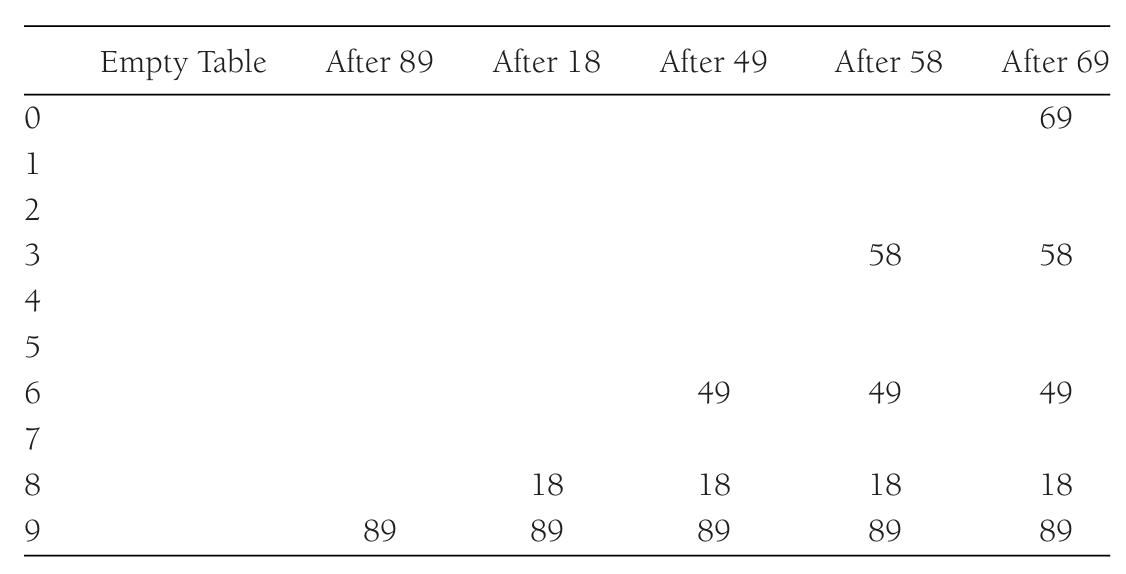
\includegraphics[width = 0.75 \textwidth]{images/double_hash.PNG}
\end{center}

当49被插入时，第一次冲突发生。$\text{hash}_2(49) = 7 - 0 = 7$，
所以49被插入到位置6。$\text{hash}_2(58) = 7 - 2 = 5$，
所以58被插入到位置3。最后，69发生冲突，并在距离$\text{hash}_2(69) = 7 - 6 = 1$处被插入。
如果我们尝试在位置0插入60，我们将会发生冲突。由于$\text{hash}_2(60) = 7 - 4 = 3$，
我们然后会尝试位置3、6、9，然后是2，直到找到一个空位。
通常可以找到一些坏情况，但这里没有太多。

正如我们之前所说，我们的示例哈希表的大小不是素数。我们这样做是为了计算哈希函数的方便，
但值得看看为什么在使用双重哈希时确保表大小为素数很重要。如果我们尝试将23插入表中，
它会与58发生冲突。由于$\text{hash}_2(23) = 7 - 2 = 5$，并且表大小为10，
我们实际上只有一个替代位置，而且它已经被占用了。因此，如果表大小不是素数，
可能会过早地耗尽替代位置。然而，如果双重哈希正确实现，模拟结果表明预期的探测次数几乎与随机冲突解决策略相同。
这使得双重哈希在理论上很有趣。然而，二次探测不需要使用第二个哈希函数，
因此在实践中可能更简单、更快，特别是对于像字符串这样的键，其哈希函数的计算成本较高。

\subsection{重新哈希}
% 5.5 

如果表变得太满，操作的运行时间将开始变得过长，对于使用二次解决的开放寻址哈希，插入可能会失败。
这可能会发生在有太多删除操作与插入操作交错进行的情况下。那么，
一个解决方案是构建另一个大约是原来两倍大的表（带有相关的新哈希函数），
然后扫描整个原始哈希表，为每个（未删除的）元素计算新的哈希值并将其插入到新表中。

\begin{figure}[htbp]
    \centering
    \begin{tabular}{|c|c|}
        \hline
        0 & 6 \\
        \hline
        1 & 15 \\
        \hline
        2 &  \\
        \hline
        3 & 24 \\
        \hline
        4 &  \\
        \hline
        5 &  \\
        \hline
        6 & 13 \\
        \hline
    \end{tabular}
    \caption{线性探测哈希表，输入为 13, 15, 6, 24}
    \label{fig:hash_table_1}
\end{figure}

作为一个例子，假设元素13, 15, 24和6被插入到一个大小为7的线性探测哈希表中。哈希函数是 $h(x) = x \mod 7$. 结果哈希表如图\ref{fig:hash_table_1}所示。

如果23被插入到表中，如图5.20所示，结果表将超过70 \% 满。因为表太满了，所以创建了一个新的表。这个表的大小是17，因为这是第一个是旧表大小两倍的素数。
新的哈希函数是 $h(x) = x \mod 17$. 扫描旧表，并将元素6, 15, 23, 24和13插入到新表中。结果表如图5.21所示。

这个整个操作被称为重新哈希。这显然是一个非常昂贵的操作；运行时间是O(N)，因为有N个元素需要重新哈希，而表的大小大约是2N，但实际上并不是那么糟糕，
因为它发生得非常不频繁。特别是，在最后一次重新哈希之前，必须有 N/2 次插入，所以它实际上为每次插入增加了一个常量成本。
这就是为什么新表的大小是旧表的两倍。如果这个数据结构是程序的一部分，这种影响是不明显的。另一方面，如果哈希是作为交互系统的一部分执行的，
那么不幸的用户，其插入操作导致了重新哈希，可能会看到速度变慢。

\begin{figure}[htbp]
    \centering
    \begin{tabular}{|c|c|}
        \hline
        0 & 6 \\
        \hline
        1 & 15 \\
        \hline
        2 & 23 \\
        \hline
        3 & 24 \\
        \hline
        4 &  \\
        \hline
        5 &  \\
        \hline
        6 & 13 \\
        \hline
    \end{tabular}
    \caption{插入 23 后的线性探测哈希表}
    \label{fig:hash_table_2}
\end{figure}

重新哈希可以通过多种方式与二次探测一起实现。一种选择是在表半满时立即重新哈希。另一种极端是在插入失败时才进行重新哈希。
第三种折中策略是在表达到某个负载因子时进行重新哈希。由于性能会随着负载因子的增加而下降，第三种策略，如果实施得好，可能是最佳的。
对于分离链接哈希表的重新哈希也是类似的。图 5.22 显示了重新哈希的实现很简单，并提供了分离链接重新哈希的实现方法。



% \subsection{基本想法}

% 让我们首先规范一下我们对数据本身结构和内存存储结构的讨论. 在我们之前的
% 讨论中, 尽管没有很明确地提出, 我们的每一个基本数据单元事实上是由两部分
% 构成的: (key, data). 这里 key 是关键字, 代表一个数据的索引. 对它最基本
% 的要求是唯一性, 也就是不同的数据, 应该有不同的 key, 显然它的一共重要功能是使数据对象具有唯一性. 
% 在一些场合, 比如二叉搜索树, 我们还要求这个 key 是有序的. 但一般来说, 有序性并不是必须的,
% 它的最基本功能是标识和区别数据, 因此唯一性就足够实现这一点. 这个 key
% 未必是数字, 它原则上可以是任何可区分的数据, 常见的有 身份ID, 车牌ID,
% 姓名(如果重名我们加额外的标识), 字符串, 数字串, 二进制串等等. 而这里的
% data 就是指被 key 唯一标识的数据本体, 是用户真正想存储的数据. 用 C++
% 的 structure 或 class 可以方便地将 key 和 data 组合成一个基本数据单位,
% 然后用某种数据结构来存储和处理. 比如, 一个学生档案, 我们可以用 (学号,
% 档案内容) 分别作为 (key, data). 因为这里学号是有序的, 我们完全可以用比如 
% AVL Tree 来管理这些档案, 并且确保每个基本操作都是 $\Theta(\log n)$. 
% 当然, 事实上这是一个不好的例子. 因为尽管学号是有序的, 但这种序在实际应用和管理中, 
% 并没有太明显的意义. 把全部学生按学号序输出? 或者寻找学号
% 最大的同学? 这种操作多少听上去有点奇怪. 因此与其用学号做 key, 可能很多
% 用户更加愿意用姓名的拼音做 key. 尽管为了解决重名问题, 我们可能需要通过
% 局部映射部分修改一些名字, 比如 zhangfei01, zhangfei02, ... .


% 我们要讨论的另一个基本问题是数据如何在内存中存储的. 比如我们将一个
% (key, data) 对称为一个 element. 比如:

% \begin{lstlisting}[language=C++]
% template <KEYTYPE, DATATYPE>
% struct Element
% {
%     KEYTYPE key;
%     DATATYPE data;
% };
% \end{lstlisting}

% 那么每一个具体的 \verb|Element| 实例, 在内存中都会占据相同的空间, 每一
% 个空间都是一段连续的内存, 由固定的字节数构成, 并且我们可以通过它的首字
% 节的内存地址访问. 也就是说, 每一个基本的数据单位, 在内存中都会占据一个
% 固定的位置, 并拥有一个固定的地址. 然后我们需要通过 \verb|key| 能访问这
% 个地址的一个索引.

% 索引本质上是从 key 到内存地址的一个映射(函数). 想一下数组的情形是什么
% 具体函数. 我们如果能构建一个计算简单的函数 (代价 $\Theta(1)$, 即与数据量无关)
% $$
% h(k) \to x,
% $$
% 这里 $k$ 代表 \verb|key|, $x$ 是一个内存地址, 且 $k \in S$, 集合 $S$
% 是全部可能的 key 构成,
% $$
% \max(h(k)) - \min(h(k)) = m,
% $$
% 直接把 $n$ 个数据, 映射到我们指定的能存放 $m$ 个连续数据的内存空间, 这里先假设 $m
% >> n$, 那么我们的一个基本操作 operator 就可以通过 operator(h(k)) 来完
% 成. 比如:
% \begin{itemize}

%   \item 判定指定的 key 是否在数据集中, search(key), 如果在, 返回内存地址,
%      否则返回 nil:

% \begin{lstlisting}[language=C++]
% if (h(key)->key != -1)
%     return h(key)->key;
% else
%     return nil;
% \end{lstlisting}

% \item 插入一个数据对 (key, data), insert(key, data):
% \begin{lstlisting}[language=C++]
% if (h(key)->key == -1)
%     h(key)->data = data;
% else
%     error(collision);
% \end{lstlisting}

% \item 删除一个已经在数据集中的数据对 (key, data), delete(key):
% \begin{lstlisting}[language=C++]
% if (h(key)->key != -1)
%     h(key)->key == -1;
% else
%     error(double deletion);
% \end{lstlisting}
% \end{itemize}

% 于是似乎我们已经完成了全部操作, 但是这里其实有严重的问题:

% \begin{enumerate}
% \item 上述方案中, 用于存放数据的连续空间的大小 $m$ 是事先给定的, 而数据集
%    的大小 $n$ 则是不断增长的. 因此终将会有一天, 数据集的大小会超过
%    $m$, 此时, 不再会有新的空间供插入, 一旦再有插入, 就必然会出现两个数
%    据抢一个地址的情形. 所以 $m >> n$ 是不存在的, 这种情形无法避免, 
%    被称为碰撞(collision);
% \item 我们没有讨论 $h$ 应该如何构建. 由于碰撞不可避免, 因此我们的构建基
%     本原则就不是避免碰撞, 而是如何提高内存的利用效率, 并且当碰撞发生时,
%     如何解决;
% \item 不论 2 采用何种策略解决碰撞, 我们必须确保这种碰撞解决策略不会影响我
%    们的删除操作的一致性和效率;
% \end{enumerate}

% 我们必须解决这些问题, 才能使哈希表成为一种实用的数据结构.

% \subsection{Hash 函数}

% 我们首先考虑如何构建哈希函数 $h(k) \to \{0, 1, \cdots, m - 1\}$. 本质上, 
% 这么做就是把存储区域看作一个数组. 这在实际应用中也是常见的. 我们称 $m$ 为槽位 (slot). 
% 这里 $k \in S$, 而 $S$ 是全部可能的键值集合, 一般认为是一个无限集, 比如, 
% 自然数全体, 或者, 全部可能的人名的拼音, 等等.

% \subsection{哈希函数的设计}

% {\bf 目标:} 

% \begin{enumerate}
% \item 将键值均匀分布到全部插槽中;
% \item 键值本身的分布特性不应影响槽位的分布. 
% \end{enumerate}

% 第二点的意思是, 比方说, 如果全部键值都是偶数 (我们在跟踪时已经注意到, 
% 所有的内存地址实际上都是偶数), 那么哈希函数的值在奇偶性上不应该不平衡. 
% 最坏的情况就是哈希的值也全是偶数, 那么天然就丢失了一半的存储空间. 
% 满足上两点最自然的想法就是一个伪随机数生成器. 但是也要注意效率. 因为本质上, 
% 随机性在这里其实不是非常重要, 更重要的是均匀性. 所以一些上古的伪随机数生成算法, 
% 由于其简单易懂高效, 一直在这个环节被采用. 

% {\bf 除同余方法 (division method) 构建映射:}

% $$
% h(k) = k ~\mathrm{mod}~ m.
% $$
% 这里对 $m$ (注意实际槽位可以根据需要做适当的调整)的要求是不能有太小的因子, 
% 特别不能是 $2$ 的整数幂. 比如若 $m$ 是偶数, 那么当 $k$ 是偶数时, $h(k)$ 也全部时偶数. 
% 更糟的, 如果 $m = 2^r$, 则 $\mathrm{mod}~2^r$ 就等价于在二进制形式下截取了低 (右) $r - 1$ 位,
% 于是不论 $k$ 是什么数, 它都丢失了全部高 $w - r + 1$ 位, 这里 $w$ 是机器字长.

% 例如 $k_1 = 10110001110111010$, $k_2 = 10001110011011010$, $r = 6$, 则
% $$
% h(k_1) = h(k_2) = 11010.
% $$
% 所以 $m$ 一般可取一个不太小的质数. 这个方法的优点是简单 (或者你临时能想起), 但缺点是昂贵. 
% 因为 $\mathrm{mod}$ 运算的代价比四则基本运算更高. 

% {\bf 乘同余方法 (multiplication method):}

% 假设槽位有 $m = 2^r$ 个, 计算机字长是 $w$, 比如 $w = 32$ 或 $64$. 则
% $$
% h(k) = (A * k ~\mathrm{mod} ~2^w) >> (w - r),
% $$
% 其中 $A$ 是满足
% $$
% 2^{w - r} < A < 2^w
% $$
% 的一个奇数, $>>$ 是右移运算. 注意 $A$ 不能太接近 $2$ 的整数次幂. 这里
% $\mathrm{mod}~2^w$ 就是取该数的低 $w$ 位, 如果机器字长就是 $w$, 
% 那么实际上什么也不用做, 自然溢出就行了. 也就是说这里其实只要控制 $A * k$ 在同样的机器字长下, 
% 比如都是标准 \verb|int| , 那么结果也溢出成一个标准 \verb|int| 就可以了, 
% 注意要 \verb|unsigned|. 而右移运算也是非常高效的基本运算, 同时右移保留了高位而不是低位, 
% 避免了之前被 $2^r$ 整除出现的浪费高位的情形. 因此整个映射效率极高且有效. 
% 历史上曾经长期采用这个方法来产生伪随机数, 直到发现它在随机性上有致命缺陷. 
% 但是它仍然具有足够好的一维均匀性(它在高维分布上会失去均匀性), 完全可以用在哈希映射的场合. 
% (目前的伪随机数算法是这个算法的一个改进, 主要基于 MT19937 算法.)

% 例: $m = 8 = 2^3$, $w = 7$, $r = 3$, $A = 1011001$, $k = 1101011$, 
% $$
% A * k = 10010100110011,
% $$
% 自然溢出后为 $0110011$, 然后右移 $w - r = 4$, 也即只保留高 $3$ 位, 因此有
% $$
% h(k) = 011.
% $$

% 我们举个例子, 比如我们这个教室大约有 150 个座位. 然后大家进来的时候都是随机找座位的, 
% 只要哪里空就坐哪里. 这样的算法, 首先是寻找座位是你必须一个个看过去, 直到找到一个空着且你能接受的位子.
% 其次是如果我们现在要找一个同学, 但是不能直接喊他的名字, 那么我们也得一个个找过去. 所以我们说, 
% 目前的算法, 在插入和查找两个基本操作上, 都是 $\Theta(m)$ 的. 这里 $m$ 是座位总数.

% 现在我们修改我们的算法, 我们给这个教室定一个规矩, 每个同学进来以后, 只许坐在 $\mbox{学号} \mod m + 1$ 的座位上.
% 这样每个同学进来以后都可以不再犹豫, 直奔他的座位. 此外如果我们要找一个具体学号的同学, 只要计算一下他的座位号, 
% 就可以直接找到他. 所以可以说, 通过加同余 Hash, 我们将插入和查找的效率都提升到了 $\Theta(1)$.

% 但是, 大家马上就会想到, 因为谁都有可能进入这个教室, 所以很快就会出现, 前后两个同学的学号 $\mod m$ 之后是同一个数. 
% 于是后面的同学会发现他的座位已经被占据了. 

% 因为我们既然是维护一张动态表, 不能假设已经知道了全部键值, 总还有新的键值会出现并需要插入. 
% 这里定义之外的约束是, 我们要求 $h$ 的像的分布尽可能均匀, 也就是尽可能平等地使用全部插槽. 
% 然而, 我们的定义并没有排斥 $h(k_1) == h(k_2)$, $k_1 \neq k_2$ 的情况. 也就是说, 
% 发生了碰撞 (collision). 碰撞可能发生在任何时候, 而且随着 $n$ 增加, 碰撞发生的可能会越来越大, 
% 并逐渐趋于必然发生(此时哈希表效率会非线性下降). 但我们首先讨论, 既然碰撞是不可避免的, 当碰撞发生时, 如何解决.

% \subsection{链接法(separate chaining)}

% 在实际操作中, 一张动态表时逐步增长起来的. 因此发生碰撞的实际情景是, 当我们试图插入一个新记录 
% \verb|k2| 时, 我们计算 $h(k_2) = i$, $i \in \{0, 1, \cdots, m - 1\}$, 
% 因此它应该存放在 \verb|T[i]|, 此时我们发现, \verb|T[i] != nil|. 因为之前已经有一条记录 $k_1 \neq k_2$, 
% 也满足 $h(k_1) = i$. 后一个判定即表明哈希碰撞已经发生. 而一个解决的思路, 就是在每一个槽位中都存放一个链表, 
% 而将所有映射到同一个槽位的记录都按插入先后次序加入链表. (后一个同学坐前一个同学腿上???)

% 这个做法直接了当, 关键的问题时效率如何? 

% {\bf 最坏情形:} $\forall k \in U$, $h(k) = i$. 

% 所有的键值都映射到同一个槽位. 那我们就得到一个链表. 于是 \verb|Search| 的效率是 $O(n)$.

% {\bf 最好情形:} 假设全部键值随机均匀独立地映射到 $\{0, 1, \cdots, m - 1\}$, 即
% $$
% h(s) \sim U\{0, 1, \cdots, m - 1\}.
% $$
% 这里 ``独立'' 指两次映射之间互相不会有任何影响. 这种情况, 有个名称叫
% {\bf 简单均匀哈希 (simple uniform hashing)}. 这是一种前提条件的假设. 在这种假设下,
% $$
% P\{h(k) = i\} = \frac{1}{m}, i \in \{0, 1, \cdots, m - 1\}.
% $$
% 而对一个 \verb|Search| 操作而言, 当它找不到目标键值, 最终返回 \verb|nil|, 
% 所需的平均（期望）时间是
% $$
% E[T] = \Theta(1 + \frac{n}{m}).
% $$
% 这里, 找到一个槽位需要 $\Theta(1)$ 的时间, 而遍历这个槽位的链表需要
% $\Theta(\frac{n}{m})$ 的时间. 我们记
% $$
% \alpha := \frac{n}{m}
% $$
% 为哈希表的装载因子 (load factor), 它代表了每个槽位平均能装多少条记录.
% 那么当 $\alpha = \Theta(1)$ 时, 有 $E[T] = \Theta(1)$.
% 但注意随着哈希表不断扩大, $n$ 不断增大, 而 $m$ 在一段时间内是不变的,
% 装载率 $\alpha$ 势必会本质超过 $1$, 此时哈希表的效率就会非线性下降. 

% 这里还有一个奇怪的地方, 在之前的算法分析中, 我们始终强调, 重要的是最坏情形, 
% 而非最好情形. 但在这里, 我们以上分析都依赖最好情形的假设. 这里的本质原因是, 
% 对于哈希表, 能否总是拿到最好情形的关键: Hash 函数是否足够均匀. 

% 回到我们的教室例子. 如果我们的教室足够大, 比如蒙民伟楼那样, 有 400 多个座位, 
% 使用的同学仍然只有我们这么多. 那么我们能否彻底避免碰撞呢? 回答是否定的, 
% 因为这是一个概率问题. 但对于这种情况, 现实中发生碰撞我们会如何处理? 
% 比如后一个同学跑到自己的座位上, 发现已经坐了一个同学, 而且他们两个都没有算错. 
% 那么他显然最自然的做法是, 再找一个空着的座位, 而不是直接坐在第一个同学腿上. 

% 或者说, 对装载率足够低的情况, 另外一种解决碰撞的思路是不构建链表, 而是构建一个哈希函数列:
% $\{h_0, h_1, \cdots, h_{m - 1}\}$. 我们要求对相同的 $k$, 不同的 $h$ 应该有不同的结果(相当于多次计算座位), 
% 因此至多 $m$ 个哈希函数. 当我们在某一次哈希操作时, $h_i(k)$ 的返回值所指向的地址如果不是 
% \verb|nil|(已被使用, 探测到碰撞发生), 那么我们再用 $h_{i + 1}(k)$ 试一次, 直到成功.

% 这种哈希设计的初衷就是不想用链表这么复杂的设计, 所以每个槽位之多只能容纳一个记录, 
% 即低装载率. 而对基本操作:

% \verb|Insert|:

% 我们从 $h_0(k)$ 开始, 寻找最小的 $i$ 使 \verb|T[|$h_i(k)$\verb|]|$==$
% \verb|nil|, 然后把 $k$ 放在 \verb|T[|$h_i(k)$\verb|]| 中;

% \verb|Search|:

% 我们从 $h_0(k)$ 起, 寻找 \verb|T[|$h_i(k)$\verb|]==|$k$(按规则计算出来的座位上确实坐着要找的同学), 
% 如果找到, 返回 $h_i(k)$ (实际上此时应该返回以 $k$ 为键值的数据); 如果出现
% \verb|T[|$h_i(k)$\verb|]==nil|(一直找到一个空座位还没有找到要找的同学), 
% 则返回 \verb|nil|(没找到). 

% 然而这种设计对于 \verb|Delete|, 会遇到困难. 比如 
% $$
% h_3(k_1) = h_2(k_2) = 5, 
% $$
% 于是在插入 $k_1$ 时, 我们可能通过 $4$ 次探查, 最终将它放在 \verb|T[5]|. 
% 然后在插入 $k_2$ 时, 我们的第 $3$ 次探查会发现碰撞, 因为 \verb|T[5]| 已经有内容了, 
% 于是我们进行了第 $4$ 次探查, 发现 $h_3(k_2) = 7$, 而 \verb|T[7] ==nil|, 
% 于是将 $k_2$ 放在了 $T[7]$, 现在我们如果要查找 $k_2$, 正确的做法是不断探查, 
% 直到发现 \verb|T[|$h_3(k_2)$\verb|] ==|$k_2$(实际是指向键值为 $k_2$的记录, 
% 讲道理会在探查到 $h_3$ 时找到). 但是假设这里我们将 $k_1$ 删除了, 
% 于是现在 \verb|T[5] == nil|, 结果导致当搜索 $k_2$ 时, 会在第 $3$ 次探查时报告 
% \verb|nil|, 最终返回一个错误的 \verb|nil| 结果. 
% 即同学 C 找了 $3$ 才找到自己的作为 100 号. 之前 2 次返回的结果是 13 号, 250 号, 
% 分别坐着同学 A 和 B. 然后突然同学 B 有事走了. 结果一个来找同学 C 的老师, 用同样的 Hash 
% 列查看第一个可能的座位 13 号, 发现上面是同学 A, 然后再看下一个 250 号, 发现空着, 于是他认为同学 C 
% 不在房间里.

% 这个问题的解决办法是:

% \begin{enumerate}
% \item 不提供删除; 
% \item 或者, 专门构建一个标志删除的键值 \verb|Deleted|. 当删除一个键值时, 
% 在原先的位置标记 \verb|Deleted|, 搜索动作不会因为 \verb|Delete| 中断, 
% 但允许插入操作往标记为 \verb|Deleted| 的槽位里插入新数据. 人可以走, 但走的时候座位上留个标记, 表示之前坐过. 
% 于是老师就会继续找下一个可能的位置. 这个有标记的座位并不影响新同学坐上去. 
% \end{enumerate}

% 开放寻址法是否成功的关键在于哈希函数序列的构建, 下面介绍几种常见的手段. 可以想象, 它的基本构建逻辑, 
% 应该类似前面的伪随机数.

% {\bf 线性探查(linear probing)}

% 令
% $$
% h(k, i) = (h(k, 0) + i) ~ \mathrm{mod} ~ m.
% $$

% 优点: 简单, 实现方便, 本质上它只有一个哈希函数 $h(k, 0)$. 

% 缺点: 存在群集现象 (primary clustering). 假设有一段连续的槽位 $i$, $i
% + 1$, $\cdots$, $i + s$ 已经被占据了, 假设 $h(k_1, 0) = i$, 那么必须经过 
% $h(k_1, 0)$, $h(k_1, 1)$, $\cdots$, $h(k_1, s)$ 才能穿过这片密集区域. 
% 而且随着槽位越来越满, 出现这样区域的概率会越来越多. 也就是说, 即便在 $\alpha < 1$ 时, 
% 也可能会局部出现这种群集现象, 导致存储效率下降. 因此线性探查虽然简单, 但只能是一个临时措施. 
% 不是一个好的解决方案.

% {\bf 二次哈希(double hashing)}

% 注意到群集现象的本源是由 Hash 的线性操作导致的, 因此我们创建非线性的 Hash.令
% $$
% h(k, i) = (h_1(k) + i * h_2(k))~\mathrm{mod}~m.
% $$
% 这里 $h_1$ 和 $h_2$ 是两个独立的哈希函数. 所以它能避免群集现象, 效果很好. 
% 一般地, 我们可以取 $m = 2^r$, 再令 $h_2$ 只产生奇数值(为什么).

% {\bf 开放寻址法的效率}

% {\bf 定理:} 若一个键值在探查完 $m$ 个可能的槽位后必然找到一个空槽($\alpha < 1$), 
% 那么在这 $m$ 个槽位中的可能探查次序共有 $m!$ 种. 现在假设这 $m!$ 
% 种探查组合实际发生的可能性都是相同且独立的. 那么
% $$
% E[\#] \leq \frac{1}{1 - \alpha}.
% $$
% 这里 $\#$ 表示探查次数. 

% \subsection{全域哈希(universal hashing)}

% 任何一个给定的哈希函数, 我们都可以认为构建一个键值集合, 使其全部映射值都相等
% (因为我们知道映射, 且无限的定义域对应有限的值域), 从而使哈希表退化为一个链表. 
% 现在的问题是如何在策略(因为开源或其他原因)暴露的情况下, 
% 保证哈希存储不被针对性攻击(敌人故意输入一串键值使你的哈希表退化, 造成效率下降). 
% 办法自然还是老方法, 随机. 不过现在对什么随机? 一个神奇的回答是, 随机挑选哈希函数. 
% 你有一个哈希函数集合, 每次在实际构建哈希表时, 都从中随机抽取一个来实现.
% (当然敌人不具有动态跟踪内存的权限, 如果敌人都有这个权限了, 做什么都没有用.)
% 由这个概念, 我们引出全域哈希的概念.

% {\bf 定义:} 设 $\mathscr{H}$ 为由有限个函数组成的集合. 称 $\mathscr{H}$ 是全域的, 
% 若 $\forall x, y \in U$, $h \in \mathscr{H}$, $x \neq y$, 满足 $h(x) = h(y)$ 
% 的函数 $h$ 至多只有 $\frac{|\mathscr{H}|}{m}$ 个. 其中
% $|\mathscr{H}|$ 表示 $\mathscr{H}$ 中的函数个数. 

% 这个定义表示 $\mathscr{H}$ 中的函数, 平均性能都很好. 或者说, 若从 $\mathscr{H}$ 
% 中随意抽取一个函数来做哈希函数, 任取两个键值, 发生碰撞的概率不超过 $\frac{1}{m}$. 
% 进而有以下定理:

% {\bf 定理：} 若 $h$ 是从 $\mathscr{H}$ 中随机抽取, 且将 $n$ 个关键字映射到一个长度大小为 
% $m$ 的表中. 则此过程中和一个指定键值发生碰撞的期望次数是
% $$ 
% E[\#] \leq \frac{n}{m} = \alpha.
% $$
% 这个说明全域哈希能达到装载率允许效率的上界, 是最优的.

% {\bf 一种构建策略}

% 令 \verb|T| 的总槽位数 $m$ 为质数, 且全体可能的键值, 都可以被转化为 $r +
% 1$ 位 $m$ 进制表示: 
% $$ 
% k = <k_0 k_1 \cdots k_r>_m, 
% $$
% 其中 $0 \leq k_i \leq m - 1$, $i = 0, 1, \cdots, r$.

% 令 $a$ 是一个随机选取的 $r + 1$ 位 $m$ 进制随机数: 
% $$
% a = <a_0 a_1 \cdots a_r>_m,
% $$
% 定义哈希函数如下:
% $$
% h_a(k) = (a, k)~\mod~m,
% $$
% 其中
% $$
% (a, k) = \sum_{i = 0}^r a_i k_i.
% $$
% 注意这里, $|\mathscr{H}| = m^{r+1}$.
% 因为每一位 $a_i$ 都有 $m$ 种取法, 共有 $r + 1$ 位 $a_i$.
% 可以证明这是一种全域哈希.
% (相当于每次建表, 都动态随机生成一个 Hash 函数或 Hash 序列, 使得敌人无法通过代码来攻击你. 
% 而且全域 Hash 的普遍性, 使得敌人也很难通过猜测你的随机参数来攻击你.)

% \subsection{完全哈希 (perfect hashing)}

% 一般我们讨论哈希表, 是将其作为一种动态数据结构讨论. 但哈希的一种应用是只用它来实现快速查表, 
% 那么能否有一种策略, 即便在最坏可能下, \verb|Search| 也是 $\Theta(1)$ 的? 
% (静态查表, 比如你有一本字典的敏感词, 你要快速判定一篇文章中是否有敏感词……)

% 解决的思路出奇的简单: 二级哈希. 也就是当碰撞发生时, 不建立链表, 而是再建立一张哈希表. 同时还要满足:

% \begin{enumerate}
% \item 两级哈希都必须是全域哈希;
% \item 第二级哈希表, 不能有碰撞.
% \item 第一级哈希表的槽位数 $m = O(n)$, 也就是装载率 $\alpha < 1$;
% \item 若第一级哈希函数在槽位 $i$ 发生了 $n_i$ 次碰撞, 那么对应 $i$ 的第二级哈希表 $S_i$, 
% 需要有槽位数 $m_i = n_i^2$.
% \end{enumerate}

% 为此, 我们需要准备一个满足全域哈希的哈希函数集. 此外, 还要求:

% 注意, 由于完全哈希是一个静态查表问题, 因此我们可以花费一定的代价建表, 
% 一旦表建成, 静态 \verb|Search| 都能实现 $\Theta(1)$ 的效率. 
% 当然这个``一定代价'', 也必须现实.

% {\bf 定理:} 若我们从全域哈希 $\mathscr{H}$ 中随机挑选一个哈希函数, 将 $n$ 
% 个键值映射到 $m = n^2$ 个槽位中, 则期望的碰撞次数
% $$
% E[\#] < \frac{1}{2}.
% $$
% 也就是说, 如果我们这样去建一张表, 在第二级哈希上, 仍然有可能发生碰撞, 
% 一旦发生碰撞, 我们可以重新抽取哈希函数, 只要抽取 $\Theta(1)$ 次, 就能在这张表上完全避免碰撞.

% \subsection{哈希表的其他应用}

% 哈希表除了作为一种存储和查找的工具, 还有一些其他的应用. 哈希映射的一个特点是将无限可能映射到一个有限的集合. 
% 从而提高检索的速度. 同时这种映射还具有均匀性. 利用这一点, 也可以在一些不太重要的验证场合使用哈希. 
% 比如说, 公司收集用户的计算机硬件信息, 不但成本高昂, 而且还有触犯隐私等法律上的风险. 
% 但是有时公司又需要在远程场合验证用户是否在使用指定的计算机. 一个限制不太严格的解决方案(如游戏, 应用软件), 
% 可以是记录用户全部硬件信息的哈希映射结果. 哈希映射结果会是一个范围一定的有限量, 可以用少量的字节就记录下来. 
% 一旦用户更改了硬件, 那么大概率会发生哈希映射值的改变. 从而感知到. 这么做的好处是效率很高, 而且并没有侵犯用户隐私. 
% 缺点当然是存在一定的哈希碰撞概率, 但是这个概率要实际发生必须是用户的硬件变化前和变化后的两次特定哈希居然发生碰撞, 
% 可以预见是一个小概率事件. 除非有黑客针对性发动``碰撞攻击''. 
% 而通过哈希函数随机抽取等技术一定程度上也可以提高安全. 当然这种方法并不适合用于密钥签名等安全性要求极高的场合. 
% 但即便对高安全性场合, 碰撞攻击也是一种常用的手段. 

\subsection{最坏情况下O(1)访问的哈希表}
% 5.7

到目前为止，我们所研究的哈希表都有一个特性，即在合理的负载因子和适当的哈希函数下，我们可以预期插入、删除和搜索的平均成本为 O(1). 
但是，假设有一个表现良好的哈希函数，搜索的最坏情况预期是什么呢？

对于分离链接，假设负载因子为 1，这是经典的球和箱问题的一个版本：给定 N 个球随机（均匀地）放置在 N 个箱子中，最拥挤的箱子中预期的球的数量是多少？
答案众所周知是 $\Theta(\log N / \log \log N)$, 这意味着平均而言，我们预期一些查询将花费接近对数时间。
对于探测哈希表中最长预期探测序列的长度，也观察到了（或可证明）类似的界限。

我们希望获得 O(1) 的最坏情况成本。在某些应用中，例如路由器和内存缓存的查找表的硬件实现，搜索具有确定的（即，恒定的）完成时间尤其重要。
假设我们事先知道 N，因此不需要重新哈希。如果我们可以在插入时重新排列项，那么对于搜索来说，O(1) 的最坏情况成本是可实现的。

在本节的剩余部分，我们描述了这个问题的最早解决方案，即完美哈希，然后是两种更近期的方法，
它们似乎提供了对多年来一直流行的经典哈希方案有希望的替代方案。

\subsubsection{完美哈希}
% 5.7.1 

假设，为了简化起见，所有 \( N \) 个元素都是预先已知的。如果一个分离链接的实现能够保证每个列表最多只有固定数量的元素，我们就完成了。
我们知道，随着我们创建更多的列表，列表平均而言会更短，因此理论上如果我们有足够的列表，那么有相当高的概率我们可能根本不会有任何冲突！

但是这种方法有两个根本问题：首先，列表的数量可能不切实际地大；其次，即使有很多列表，我们可能仍然不幸地遇到冲突。
原则上，第二个问题相对容易解决。假设我们选择列表的数量为\( M \)（即，\( \text{TableSize} \)是\( M \)）, 这足够大以保证至少有\( \frac{1}{2} \)的概率不会有任何冲突。
然后，如果检测到冲突，我们只需清空表并使用与第一个独立的不同哈希函数再次尝试。如果我们仍然遇到冲突，我们尝试第三个哈希函数，依此类推。
预期的尝试次数最多为 2（因为成功概率是\( \frac{1}{2} \)），这都计入插入成本。第 5.8 节讨论了如何生成额外哈希函数的关键问题。

所以我们剩下要确定的是列表的数量\( M \)需要有多大。不幸的是，\( M \)需要相当大；具体来说\( M = \Omega(N^2) \). 
然而，如果\( M = N^2 \), 我们可以证明表至少有\( \frac{1}{2} \)的概率是无冲突的，这个结果可以用来对我们的基本方法进行可行的修改。

\textbf{定理 5.2} 如果\( N \)个球被放入\( M = N^2 \)个箱子中，那么没有任何一个箱子包含超过一个球的概率小于\( \frac{1}{2} \).
（这里假设每个球放入每一个箱子的概率都是相同的。这是基本假设。）
\begin{proof}
  如果一对\( (i, j) \)的球被放入同一个箱子，我们称之为冲突。设\( C_{i,j} \)是任何两个球\( (i, j) \)产生的预期冲突数量。
  显然，任何两个指定的球相撞的概率是\( \frac{1}{M} \)（先按住一个，再放入同一个位置。概率由第二个决定），
  因此\( C_{i,j} \)是\( \frac{1}{M} \)，因为涉及这对\( (i, j) \)的冲突数量要么是 0 要么是 1 。
  因此，整个表的预期冲突数量是（注意 $i < j$，两个球地位对等，先放谁都一样。）
  $$
  \sum_{(i,j), i<j} C_{i,j}.
  $$
  由于有\( \frac{N(N-1)}{2} \)对（N 取 2），这个总和碰撞数是 （$N^2$ 就是为了足够苟）
  $$ 
  \frac{N(N-1)}{2M} = \frac{N(N-1)}{2N^2} < \frac{1}{2}.
  $$
  由于预期的冲突数量低于\( \frac{1}{2} \), 那么至少有一个冲突的概率也必须低于\( \frac{1}{2} \).
\end{proof} 

当然，使用\( N^2 \)个列表是不切实际的。然而，前面的分析建议了以下替代方案：只使用\( N \)个箱子，
但通过使用哈希表而不是链接列表来解决每个箱子中的冲突。这个想法是因为每个箱子预计只有几个项目，
所以用于每个箱子的哈希表可以是箱子大小的二次方。图5.24展示了基本结构。这里，主哈希表有十个箱子。
箱子1、3、5和7都是空的。箱子0、4和8有一个项目，因此它们通过一个有一个位置的二级哈希表来解决。
箱子2和6有两个项目，因此它们将被解决到一个有四个\( (2^2) \)位置的二级哈希表中。
而箱子9有三个项目，因此它被解决到一个有九个\( (3^2) \)位置的二级哈希表中。

\begin{figure}
  \centering
  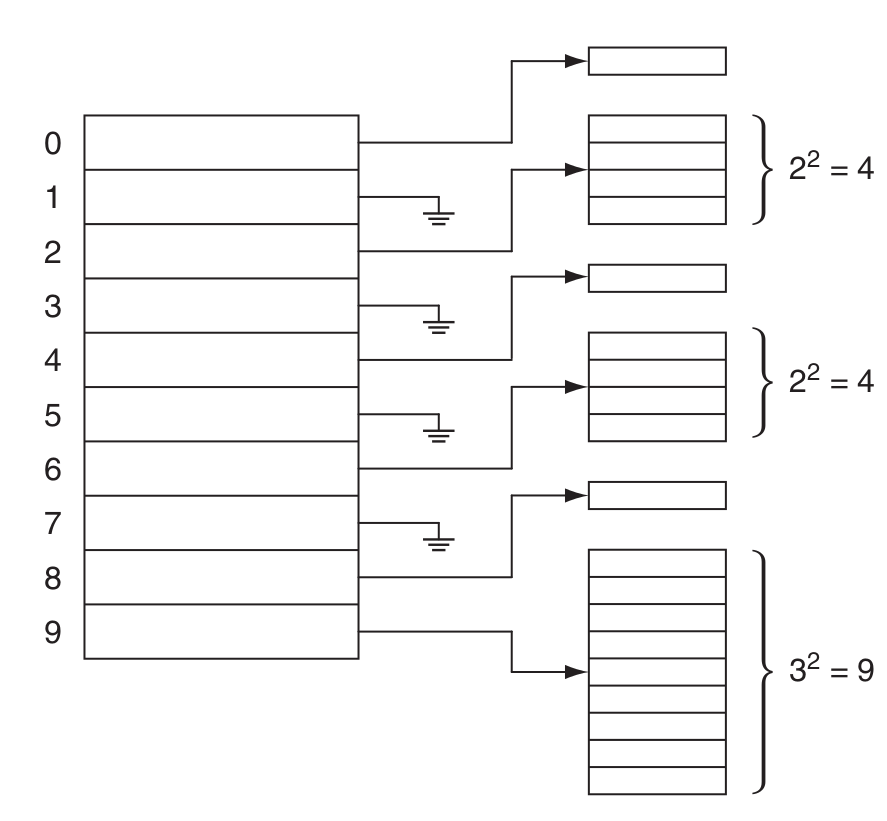
\includegraphics[width=0.6\textwidth]{images/perfect_hash.png}
  \caption{完美哈希表的基本结构 —— 二级哈希。}
  \label{fig:perfect_hash}
\end{figure}

与原始想法一样，每个二级哈希表将使用不同的哈希函数构建，直到它无冲突。如果产生的冲突数量高于所需，主哈希表也可以构建多次。
这种方案被称为完美哈希。剩下要证明的是，二级哈希表的总大小确实预期为线性。

\textbf{定理 5.3}

如果将\( N \)个项目放入包含\( N \)个箱子的主哈希表中，那么二级哈希表的总大小的期望值最多为\( 2N \).

\begin{proof}
使用与定理 5.2 证明相同的逻辑，成对冲突的预期数量最多为 \( \frac{N(N-1)}{2N} \), 或\( \frac{N-1}{2} \). 
设\( b_i \)为主哈希表中映射到位置\( i \)的项目数量；观察到二级哈希表中为此单元格使用了\( b_i^2 \)空间，
这解释了\( b_i(b_i-1)/2 \)次成对冲突（撞进 $i$ 的总数），我们称之为\( c_i \). 因此，第\( i \)个二级哈希表使用的\( b_i^2 \)空间是\( 2c_i + b_i \). 
（这里其实对 $b_i^2$ 做了个分解）总空间就是\( 2\sum c_i + \sum b_i \). 总冲突数是\( (N-1)/2 \)（来自本证明的第一句话）；
项目总数当然是\( N \),（分别解释了两个求和式） 所以我们得到的二级空间需求总计为\( 2(N-1)/2 + N < 2N \).

因此，总二级空间需求超过\( 4N \)的概率最多为\( \frac{1}{2} \)（否则，期望值将高于\( 2N \)）, 所以我们可以继续为主表选择哈希函数，
直到我们生成适当的二级空间需求。一旦完成，每个二级哈希表本身平均只需要两次尝试就可以无冲突。在表构建完成后，任何查找都可以在两次探测中完成。
\end{proof}
  
完美哈希适用于所有项目都预先已知的情况。存在允许插入和删除的动态方案（动态完美哈希），但我们将研究两种在实践中似乎与经典哈希算法竞争的更新的替代方案。
    
\subsubsection{5.7.2 布谷鸟哈希}

从我们之前的讨论中，我们知道在球与箱问题中，如果\( N \)个项目随机投入到\( N \)个箱子中，最大箱子的大小预期为\( \Theta(\log N / \log \log N) \). 
由于这个界限已经被知道很长时间，并且这个问题已经被数学家们很好地研究过，所以在 1990 年代中期，当显示出如果在每次投入时，随机选择两个箱子，
并将项目投入到当时更空的箱子中，那么最大箱子的大小将仅为\( \Theta(\log \log N) \), 这是一个显著较小的数字，这令人惊讶。
很快，许多潜在的算法和数据结构从这个 ``双重选择的力量'' 的新概念中产生。

其中一个想法就是布谷鸟哈希。在布谷鸟哈希中，假设我们有\( N \)个项目。我们维护两个表，每个表都超过一半是空的，
并且我们有两个独立的哈希函数，可以将每个项目分配到每个表中的位置。布谷鸟哈希保持了一个不变性，即一个项目总是存储在这两个位置中的一个。

作为一个例子，图5.25展示了一个潜在的布谷鸟哈希表，用于六个项目，有两个大小为5的表（这些表太小，但作为例子效果很好）。基于以下哈希函数：

\begin{figure}
  \centering
  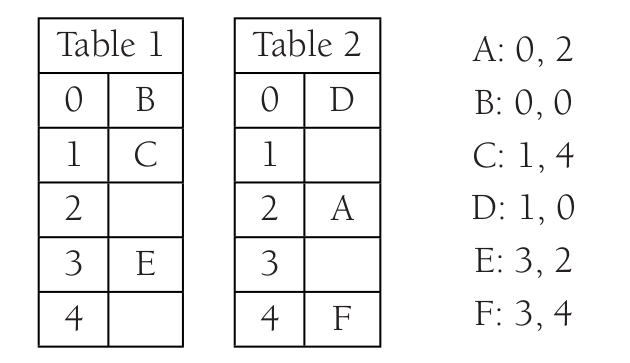
\includegraphics[width=0.6\textwidth]{images/cuckoo.png}
  \caption{图5.25 潜在的布谷鸟哈希表。哈希函数显示在右侧。对于这六个项目，在表1中只有三个有效位置，在表2中也只有三个有效位置，因此不清楚这种安排是否容易找到。}
  \label{fig:bubble_hash}
\end{figure}

随机选择的哈希函数下，项目A可以位于表1的第0个位置或表2的第2个位置。项目F可以位于表1的第3个位置或表2的第4个位置，以此类推。这立即意味着，在布谷鸟哈希表中的搜索最多需要两次表访问，而一旦找到项目，移除操作就很简单（现在不需要延迟删除）。

但是有一个重要的细节：表是如何构建的？例如，在图5.25中，对于六个项目，第一个表中只有三个可用位置，第二个表中也只有三个可用位置。因此，这六个项目只有六个可用位置，我们必须为我们的六个项目找到一个理想的槽位匹配。显然，如果有第七个项目G，其在表1的位置是1，在表2的位置是2，那么它就不能通过任何算法插入到表中（七个项目将竞争六个表位置）。有人可能会说，这意味着表的负载过高（G将产生0.70的负载因子），但同时，如果表中有成千上万的项目，并且负载很轻，但我们有A、B、C、D、E、F、G这些具有这些哈希位置的项目，仍然不可能插入所有七个项目。因此，这个方案能否奏效并不明显。在这种情况下，解决方案是选择另一个哈希函数，只要这种情况不太可能发生，这就可以。

布谷鸟哈希算法本身很简单：要插入一个新项目x，首先确保它尚未存在。然后我们可以使用第一个哈希函数，如果（第一个）表位置为空，项目就可以放置。因此，图5.26显示了将A插入空哈希表的结果。

现在假设我们要插入B，它在表1和表2中的哈希位置都是0。在算法的剩余部分，我们将使用\( (h_1, h_2) \)来指定两个位置，所以B的位置由\( (0,0) \)给出。表1的第0个位置已经被占用。此时有两个选择：一个是查看表2。问题是表2的第0个位置也可能被占用。碰巧在这种情况下它没有被占用，但标准布谷鸟哈希表使用的算法不会去查看。相反，它预先将新项目B放置在表1中。为了做到这一点，它必须替换A，所以A移动到表2，使用其在表2中的哈希位置，即第2个位置。结果如图5.27所示。很容易插入C，如图5.28所示。

接下来我们想要插入D，其哈希位置为\( (1, 0) \)。但是表1的位置（第1个位置）已经被占用。还要注意，表2的位置尚未被占用，但我们不会去查看那里。相反，我们让D替换C，然后C进入表2的第4个位置，这是由其第二个哈希函数建议的。结果表如图5.29所示。

完成这个操作后，可以轻松地插入E。到目前为止，一切都很好，但现在我们能插入F吗？图5.30到5.33展示了这个算法通过替换E，然后是A，最后是B，成功地插入了F。

显然，正如我们之前提到的，我们不能成功地插入具有哈希位置(1, 2)的G。如果我们尝试这样做，我们将替换D，然后是B，接着是A、E、F和C，然后是C。

然后它将尝试回到表1的第1个位置，替换最初放置在那里的G。这将使我们得到图5.34。现在，G将尝试在表2中的备选位置（位置2），然后替换A，这将导致B被替换，接着是D，然后是C，C会替换F，F会替换E，E现在将从位置2替换G。此时，G将陷入一个循环。

核心问题涉及到诸如防止插入完成的循环的概率是多少，以及成功插入所需的预期位移次数是多少等问题。幸运的是，如果表的负载因子低于0.5，分析表明循环的概率非常低，预期的位移次数是一个小常数，并且成功插入需要超过\( O(\log N) \)次位移的可能性极低。因此，我们可以在一定数量的位移后用新的哈希函数重建表。

检测到。更准确地说，单个插入需要一套新的哈希函数的概率可以降低到\( O(1/N^2) \)；新的哈希函数本身会产生\( N \)次更多的插入以重建表，但即便如此，这意味着重建成本是最小的。然而，如果表的负载因子达到0.5或更高，那么循环的概率会急剧上升，这个方案不太可能很好地工作。

布谷鸟哈希发布后，提出了许多扩展。例如，我们可以使用更多的表，如3个或4个，而不是两个表。虽然这增加了查找的成本，但它也极大地提高了理论空间利用率。在某些应用中，通过独立的哈希函数进行的查找可以并行完成，因此几乎不需要额外的时间。另一个扩展是允许每个表存储多个键；同样，这可以增加空间利用率，使插入更容易，并且更有利于缓存。如图5.35所示，有各种可能的组合。最后，布谷鸟哈希表通常被实现为一个巨大的表，带有两个（或更多）哈希函数，这些函数探测整个表，一些变体尝试在第二个哈希表中有可用位置时立即放置一个项目，而不是开始一系列位移。

\subsection*{布谷鸟哈希表实现}

实现布谷鸟哈希需要一组哈希函数；简单地使用hashCode来生成哈希函数集合是没有意义的，因为任何hashCode冲突都会导致所有哈希函数中的冲突。图5.36展示了一个简单的接口，可以用来将哈希函数族发送到布谷鸟哈希表。

\bibliography{../bibtexlib/crazyfish.bib}
\bibliographystyle{plain}

\end{document}
